% Week 6 实验周报 —— 编译方式:XeLaTeX
\documentclass[11pt]{ctexart}
\usepackage[a4paper, margin=2.5cm]{geometry}
\usepackage{amsmath}
\usepackage{booktabs}
\usepackage{graphicx}
\usepackage{hyperref}
\usepackage{enumitem}
\setlist{nosep}

\title{\textbf{Chooser Option 定价项目 —— 第 6 周实验报告}\\
\large Model Training, Tuning \& Comparison}
\author{佟铸城 (Zhucheng Tong)}
\date{2026 年 8 月 25 日}

\begin{document}
\maketitle

\section{本周目标}
完成 Week 6 三项交付物:(1) 训练完成的模型文件;(2) 含指标的对比分析报告;(3) SHAP 特征重要性可视化。

\section{完成工作}
\begin{enumerate}
  \item \textbf{walk-forward 滚动重训框架}(\texttt{src/ml/walkforward.py}):每 63 交易日以扩张窗口重训,逐块保持 252 行净化与 scaler 重拟合;
  \item \textbf{调参}:各模型族在验证集上网格搜索(审计保证选择日志零测试信息);利率水平特征改为滚动均值偏离;MLP 输入裁剪鲁棒化;路线 B 同步锚定化;
  \item \textbf{测试集开封一次}:198 个交易日(2024-03 至 2024-12)最终评估,8 指标+综合分+权重敏感性;
  \item \textbf{SHAP}:部署版 GBDT 的 beeswarm 与重要性条形图;
  \item 部署模型已存 \texttt{models/final\_*.joblib}(7 个,含 scaler 与超参数)。
\end{enumerate}

\section{核心结果:一个如实报告的负结果}
\begin{enumerate}
  \item \textbf{测试集上没有任何 ML 配置击败 EWMA 基线}:EWMA MAE \$8.51、综合分 1.000 在四种权重方案下均列第一;最好的 ML(鲁棒化 MLP)综合分 2.02,验证集冠军 LSTM(val MAE 2.82)测试劣化至 17.07——典型的验证集过拟合;
  \item \textbf{归因三条}:(a) 锚定比率目标有强低频状态自相关,训练数据只含约一个半状态轮换,模型学到的是``上一个状态''而非可泛化规律;(b) 测试期每个标签窗口都覆盖 2025-04 关税崩盘——与第 4 周``2019 尾段''同构的不可预见事件,EWMA 胜在\textbf{不试图预测};(c) 事后诊断(如实标注、未用于选择)表明第 5 周的验证集胜利部分源于训练分布与验证需求的巧合——\textbf{单一验证窗的胜利不构成部署证据};
  \item \textbf{SHAP 与第 2 周互信息结论一致}:长窗口已实现波动率主导修正方向(均值回复逻辑),规律本身合理,但其幅度无法从一个周期的数据中稳定标定;
  \item \textbf{工具决策}:第 7--8 周双定价 = EWMA 锚定 BSM 为主定价 + ML 修正价作参考显示并附样本外警示。负结果界定了 ML 增强在当前数据规模下的适用边界,改进条件明确:多周期历史或个股隐含波动率数据。
\end{enumerate}

\begin{figure}[h!]
\centering
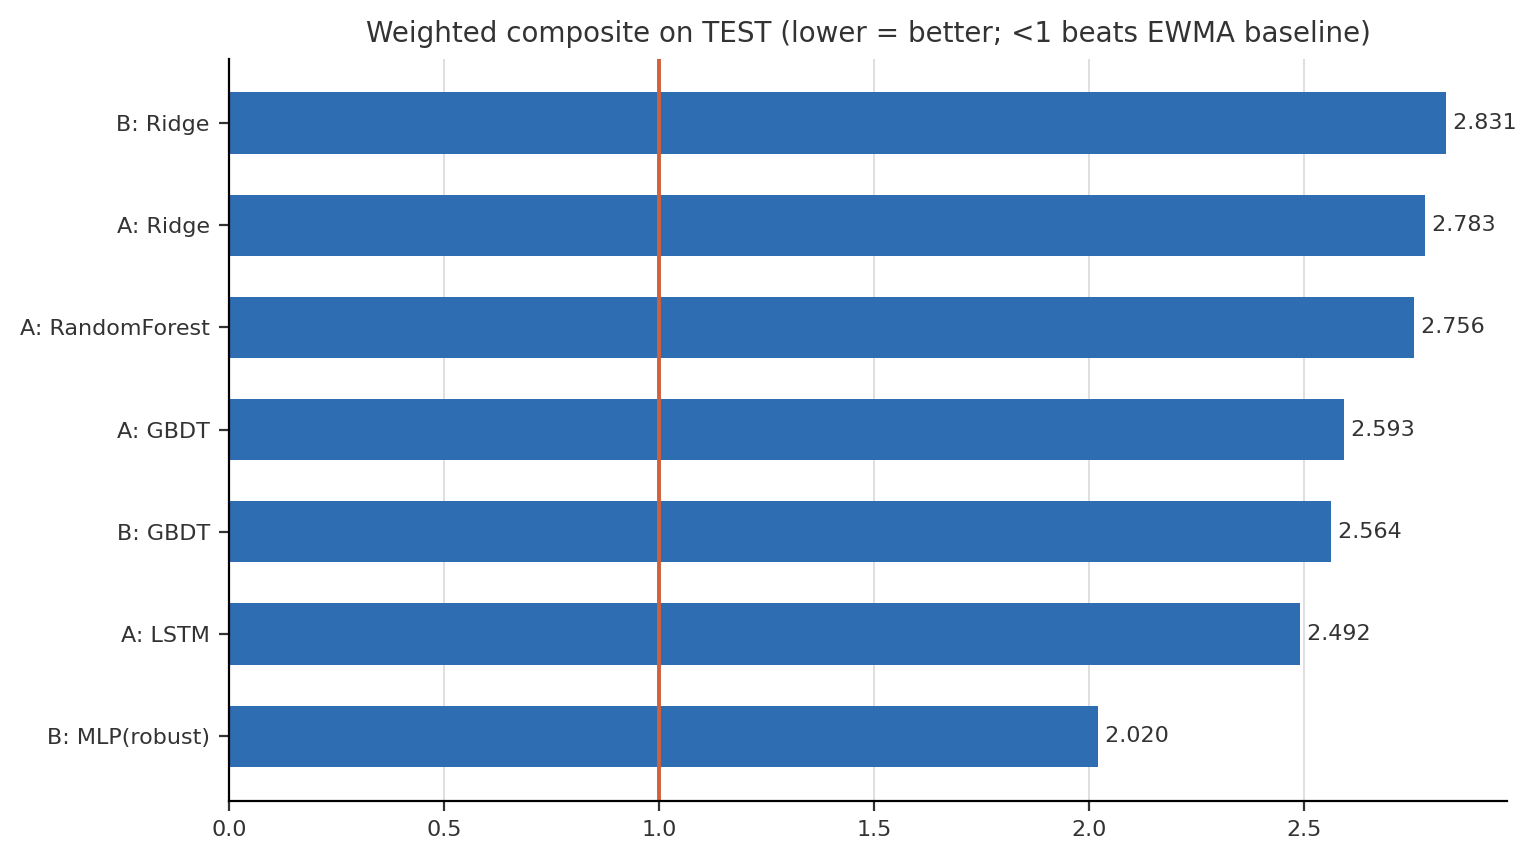
\includegraphics[width=0.74\textwidth]{../../docs/week6/figures/test_composite.png}
\caption{测试集综合分:EWMA 基线胜出}
\end{figure}

\section{实验记录}
负结果的资格审查:六项审计(净化、调参日志、确定性、综合分重算、SHAP 覆盖、解码防护)全部通过后,才将``ML 未胜出''定性为科学结论而非实现缺陷。全部数字可由 \texttt{python -m src.analysis\_w6} 一键复现。

\section{下周计划(Week 7:敏感性分析与工具开发)}
扩展敏感性分析(SHAP 化的新特征影响量化、极端情景:波动率 $+50\%$、加息 200bp)、Streamlit 定价工具框架(双定价+误差区间)、实时数据自动更新集成。
\end{document}
